\chapter{Geometric transforms}

\section{Problem statement}

Develop a geometric transform program that will rotate, translate,
and scale an image by specified amounts, using the nearest neighbor
and bilinear interpolation methods, respectively.

\section{Python implementation}

Usage:~\textbf{problem6.py [-h] -i INPUT} \\
       \textbf{(-t TRANSLATE [TRANSLATE ...] | -r ROTATE | -s SCALE)}
       \textbf{(--nearest | --bilinear) [--ntruncate] [--debug]}

Use \textbf{python problem6.py -h} to see the help.

\pagebreak

\begin{figure}[!htb]\centering
    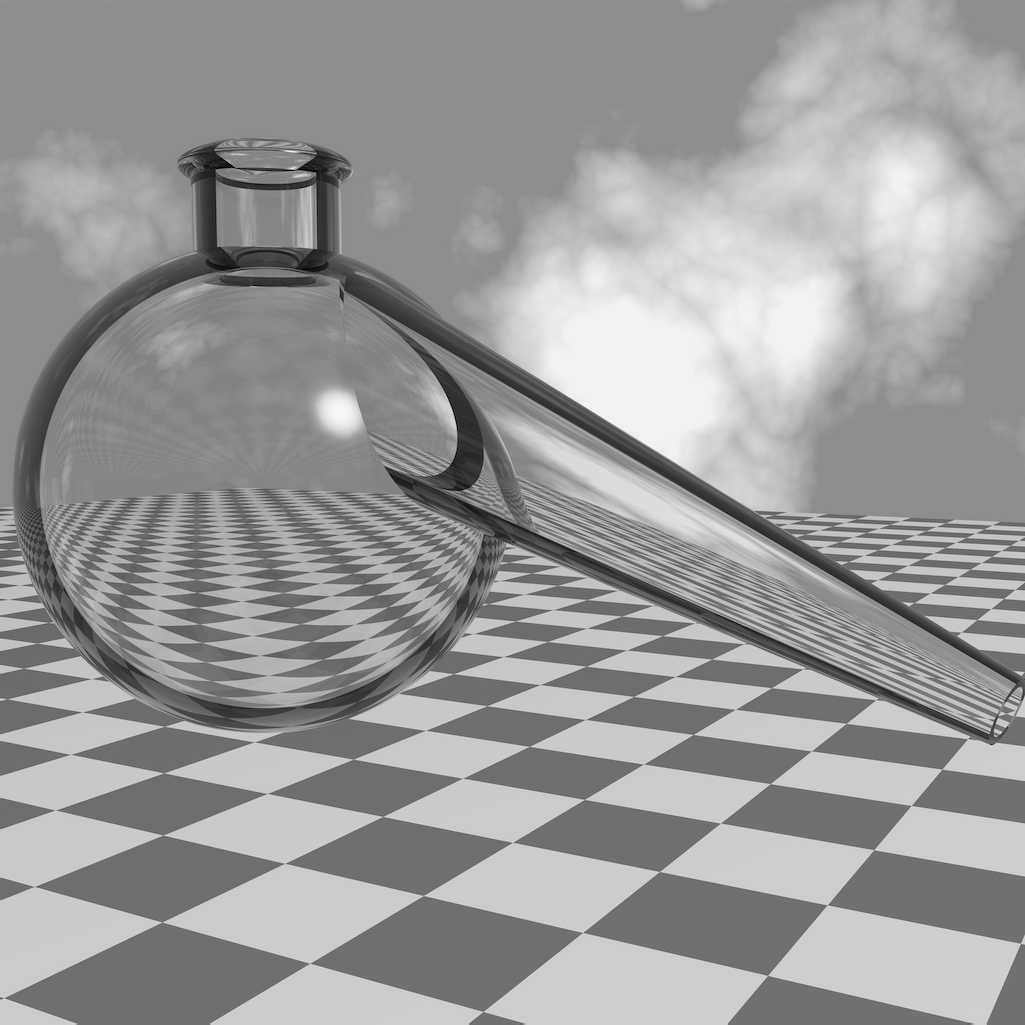
\includegraphics[width=0.6\linewidth]{./images/6/original.png}
    \caption{\small{Original image}}
\end{figure}


\pagebreak

\section{Translation}

\textbf{python problem6.py -i ray\_trace\_bottle.tif --bilinear -t tx ty}, where (tx, ty) is the 2D translation vector.

\begin{figure}[!htb]\centering
    \begin{minipage}{0.6\textwidth}
        \frame{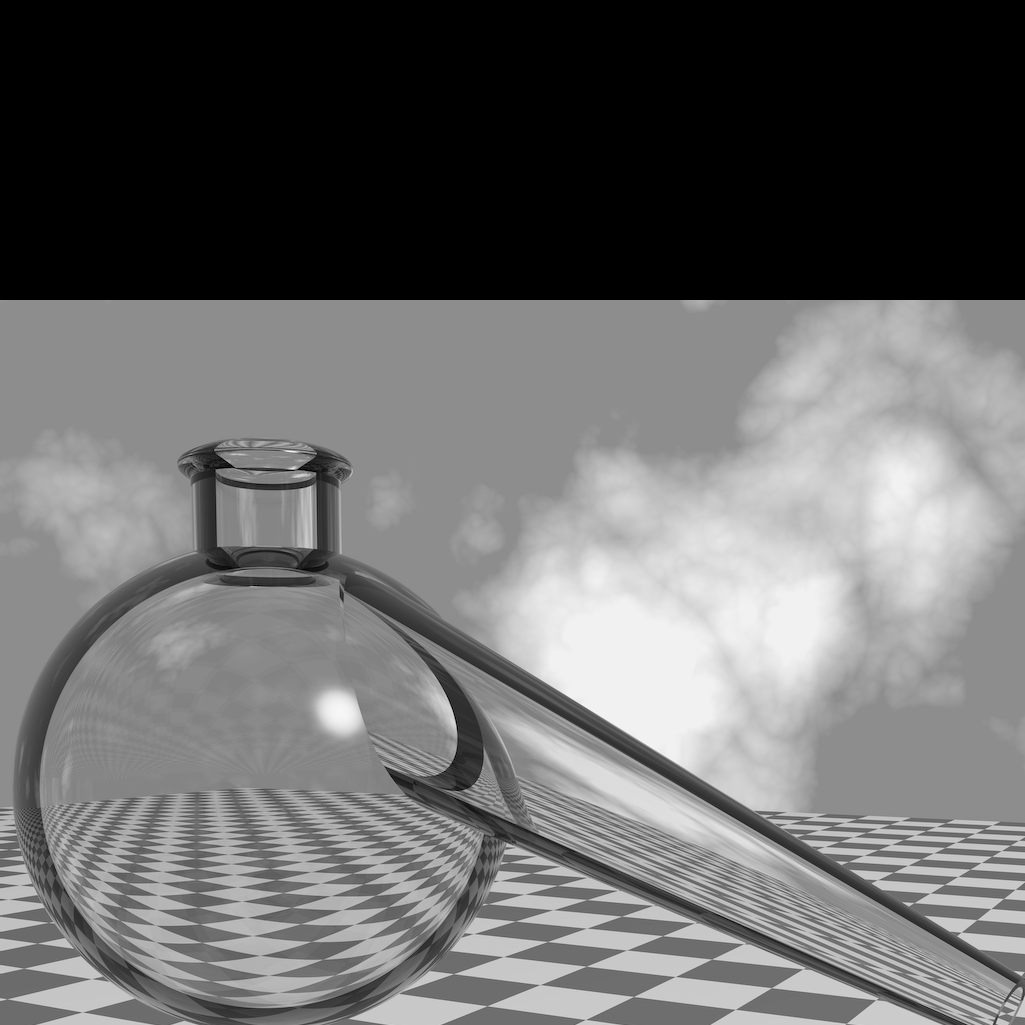
\includegraphics[width=\linewidth]{./images/6/translate_0_300_nn.png}}
        \caption{\small{Translation (0, 300) nearest}}
    \end{minipage}
\end{figure}

\begin{figure}[!htb]\centering
    \begin{minipage}{0.6\textwidth}
    \frame{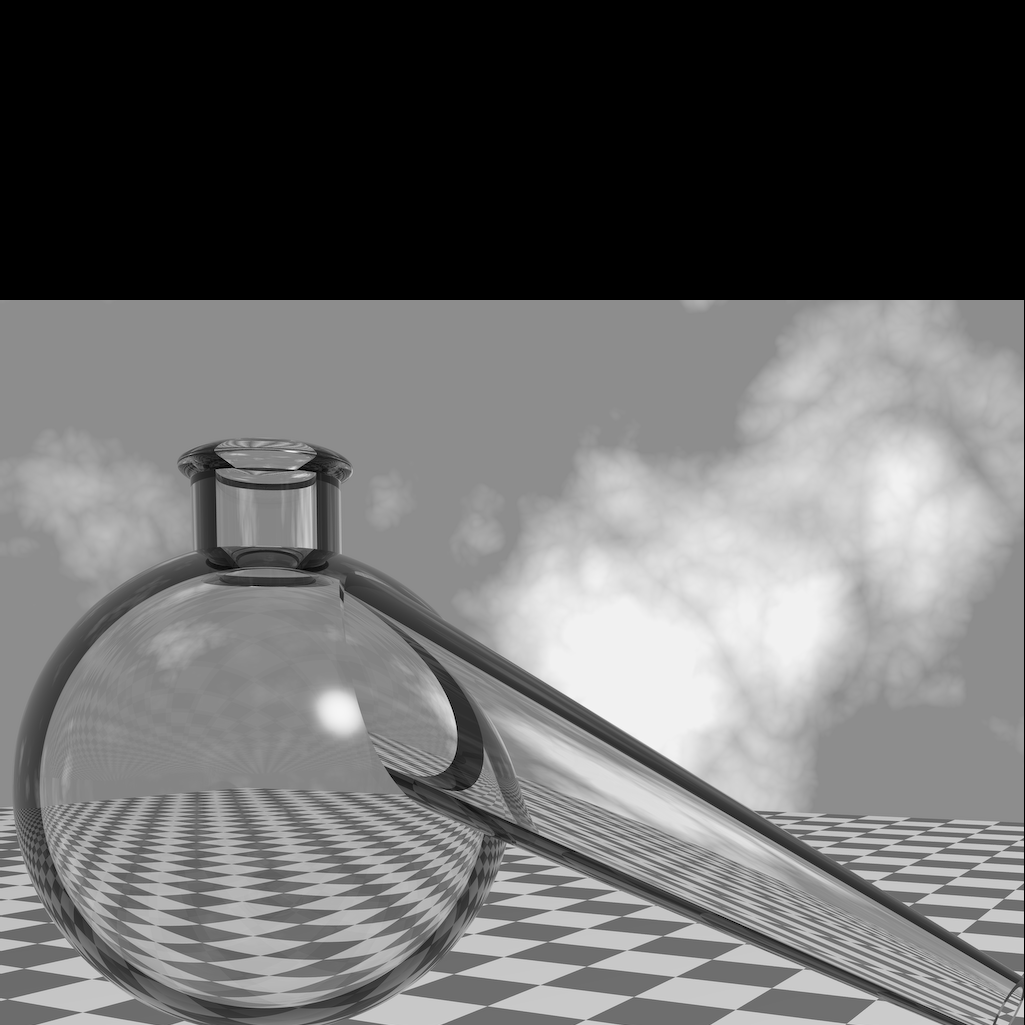
\includegraphics[width=\linewidth]{./images/6/translate_0_300_bl.png}}
    \caption{\small{Translate (0, 300) bilinear}}
    \end{minipage}
\end{figure}

\pagebreak

\begin{figure}[!htb]\centering
    \begin{minipage}{0.6\textwidth}
        \frame{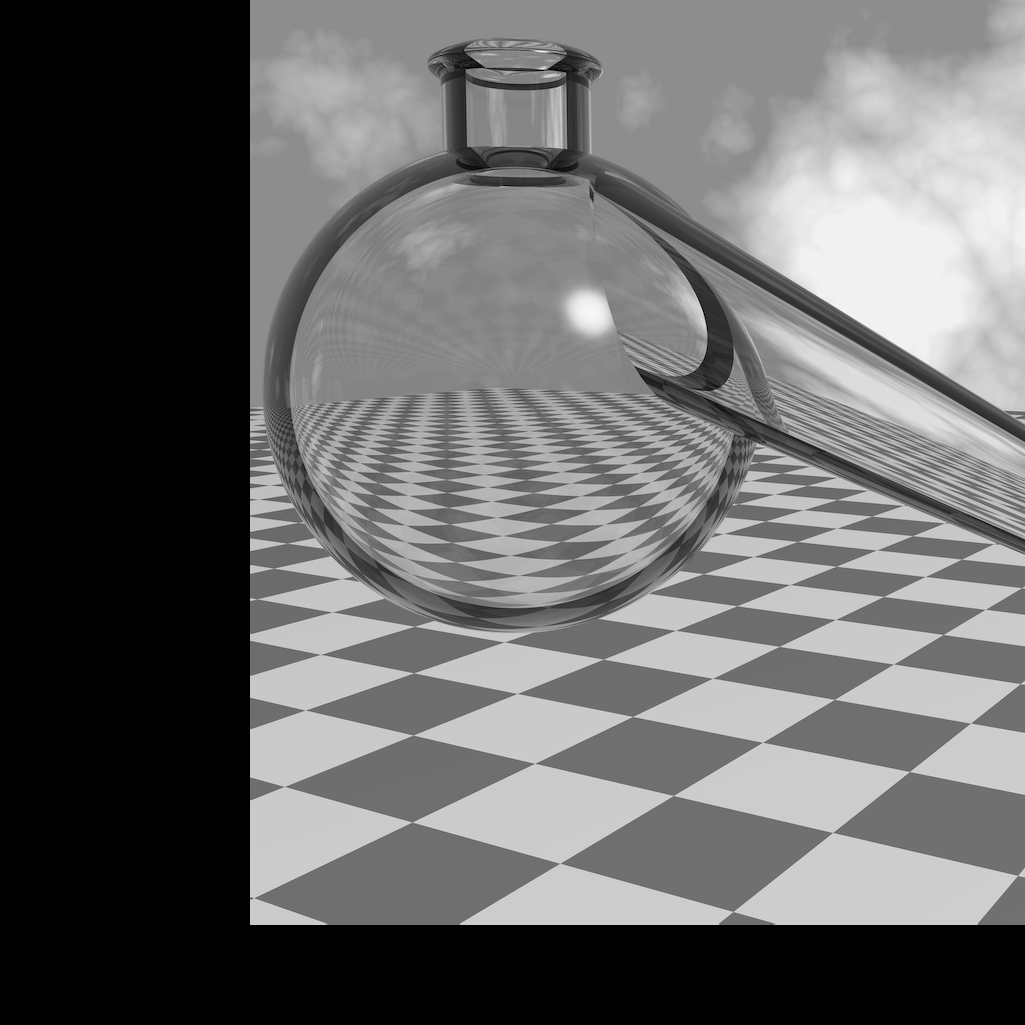
\includegraphics[width=\linewidth]{./images/6/translate_250_-100_nn.png}}
        \caption{\small{Translation (250, -100) nearest}}
    \end{minipage}
\end{figure}

\begin{figure}[!htb]\centering
    \begin{minipage}{0.6\textwidth}
    \frame{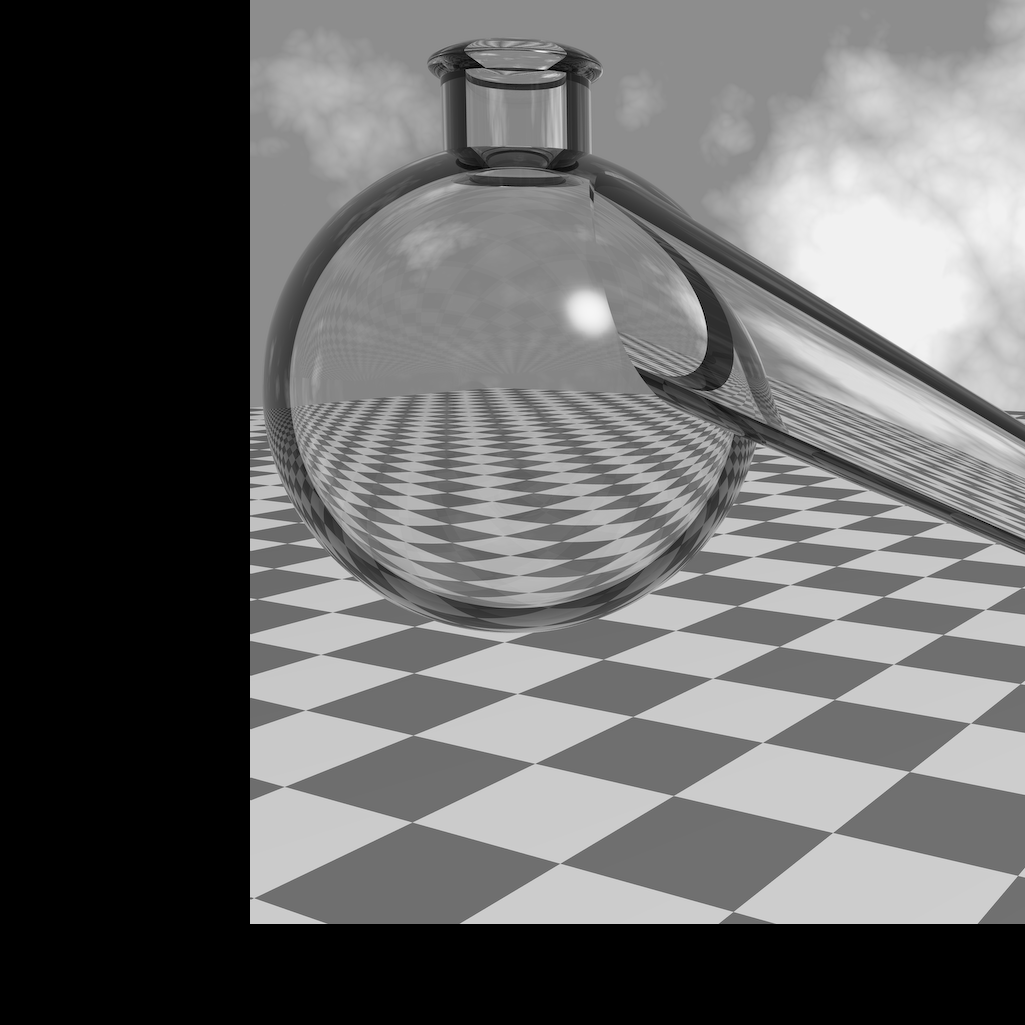
\includegraphics[width=\linewidth]{./images/6/translate_250_-100_bl.png}}
    \caption{\small{Translate (250, -100) bilinear}}
    \end{minipage}
\end{figure}

\pagebreak

\begin{figure}[!htb]\centering
    \begin{minipage}{0.6\textwidth}
        \frame{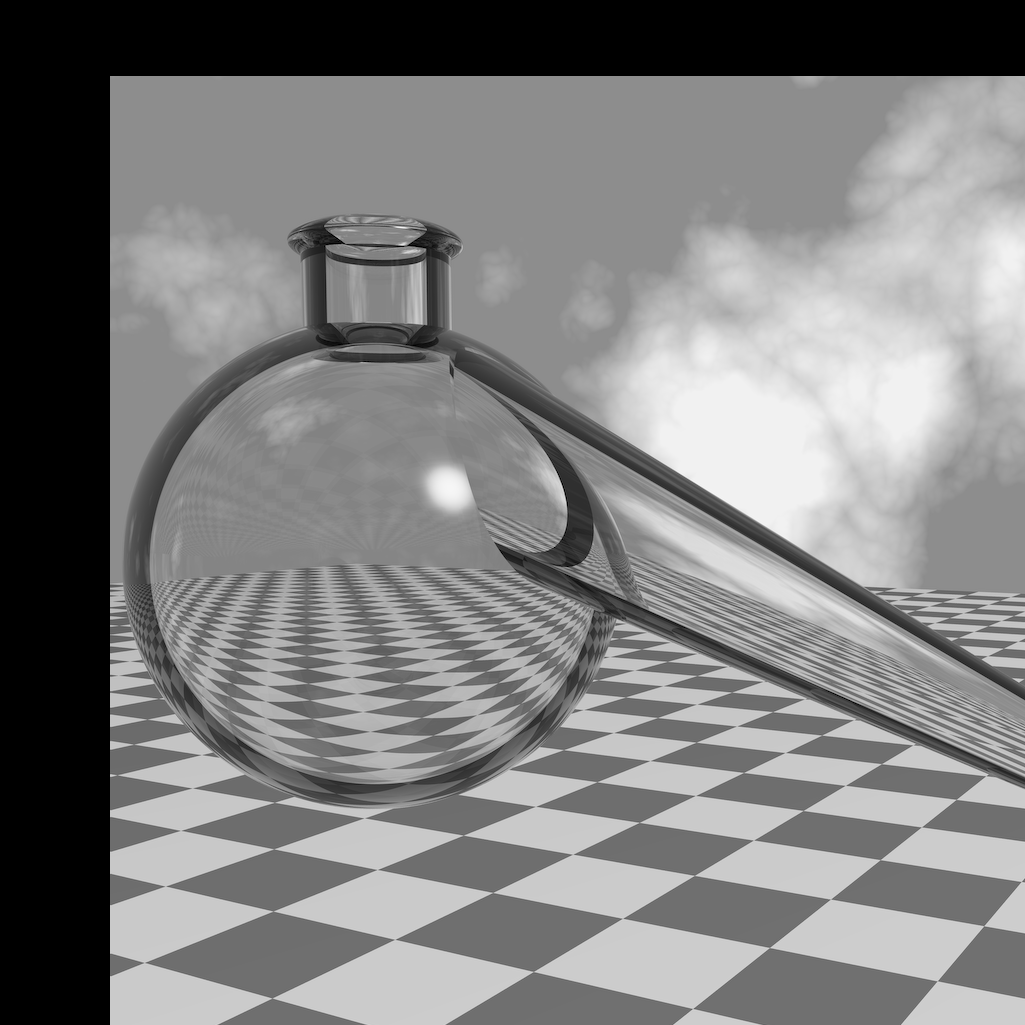
\includegraphics[width=\linewidth]{./images/6/translate_109_8_75_5_nn.png}}
        \caption{\small{Translation (109.8, 75.5) nearest}}
    \end{minipage}
\end{figure}

\begin{figure}[!htb]\centering
    \begin{minipage}{0.6\textwidth}
    \frame{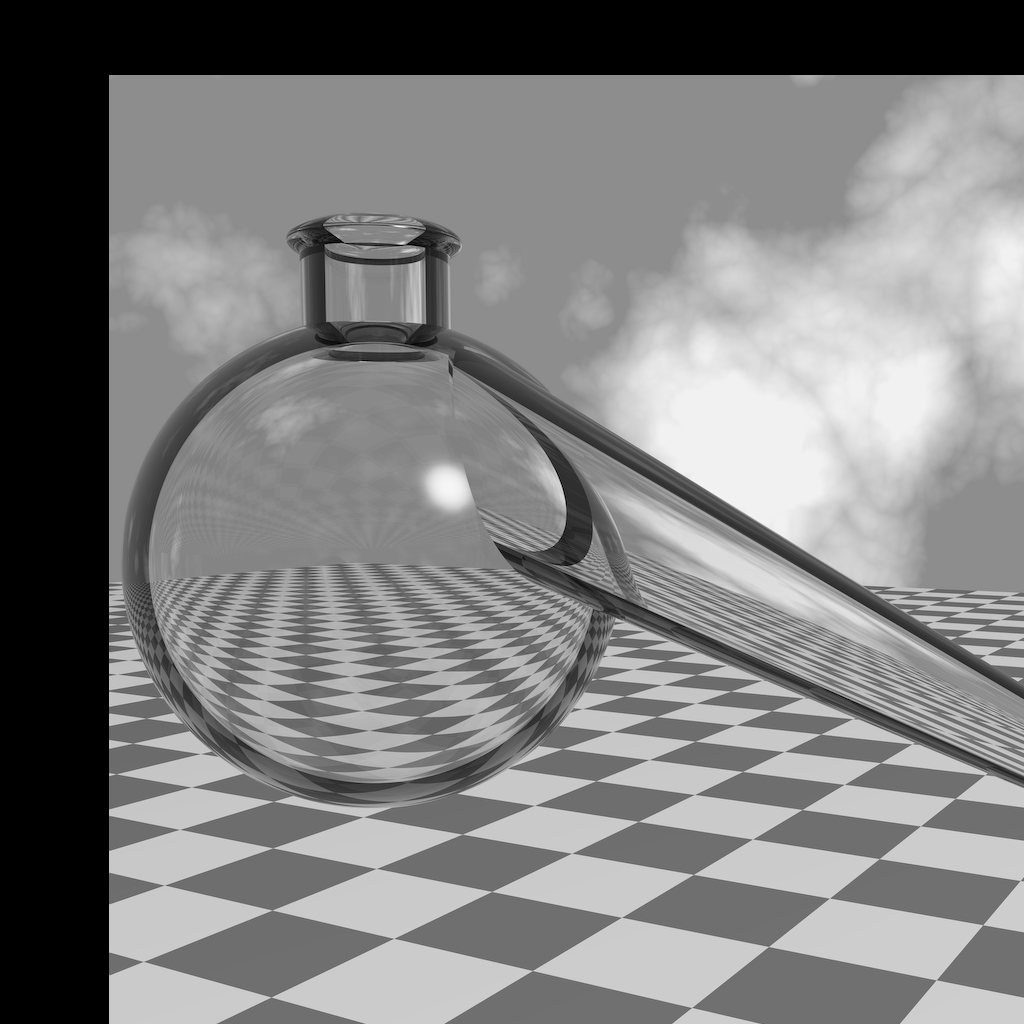
\includegraphics[width=\linewidth]{./images/6/translate_109_8_75_5_bl.png}}
    \caption{\small{Translation (109.8, 75.5) bilinear}}
    \end{minipage}
\end{figure}


\pagebreak

\section{Rotation}

\textbf{python problem6.py -i ray\_trace\_bottle.tif --nearest -r theta}, where theta is the angle of rotation.

\begin{figure}[!htb]\centering
    \begin{minipage}{0.6\textwidth}
        \frame{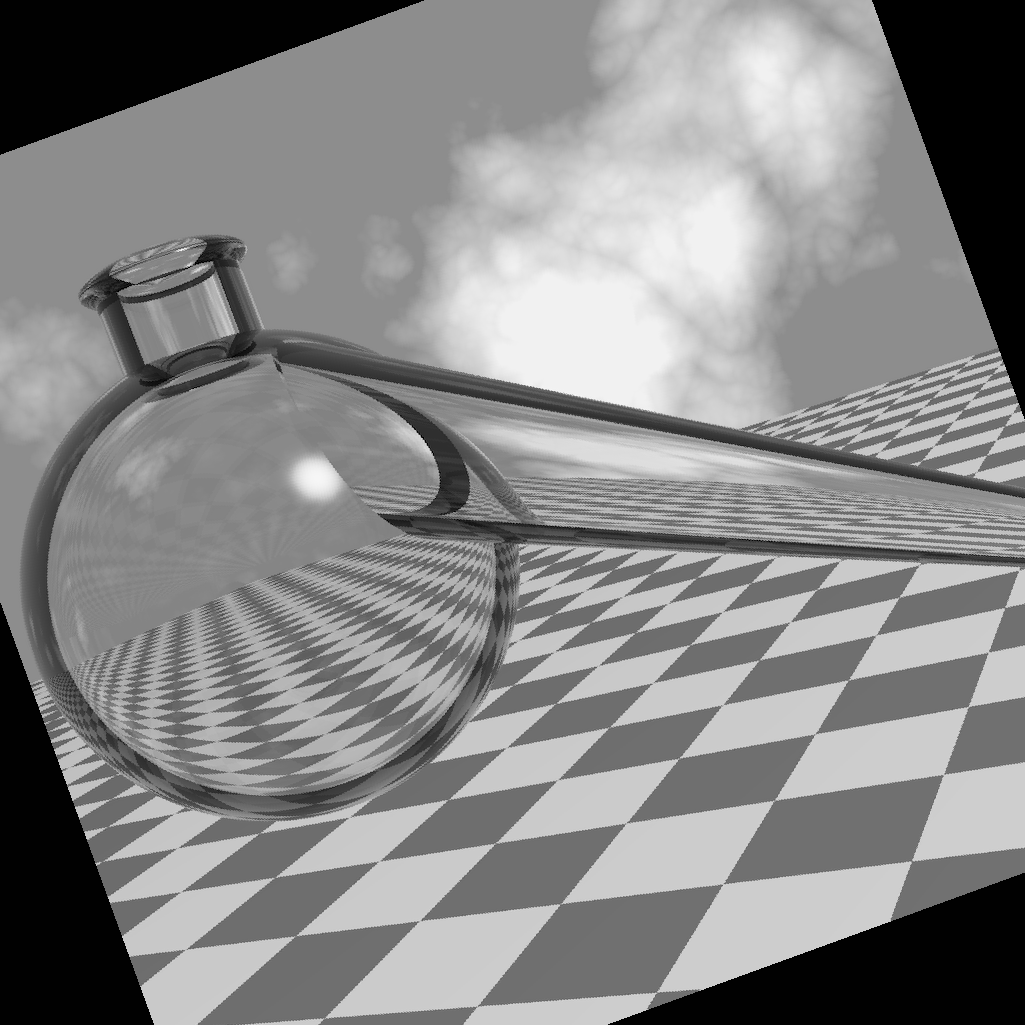
\includegraphics[width=\linewidth]{./images/6/rotate_20_nn.png}}
        \caption{\small{Rotate 20° nearest}}
    \end{minipage}
\end{figure}

\begin{figure}[!htb]\centering
    \begin{minipage}{0.6\textwidth}
    \frame{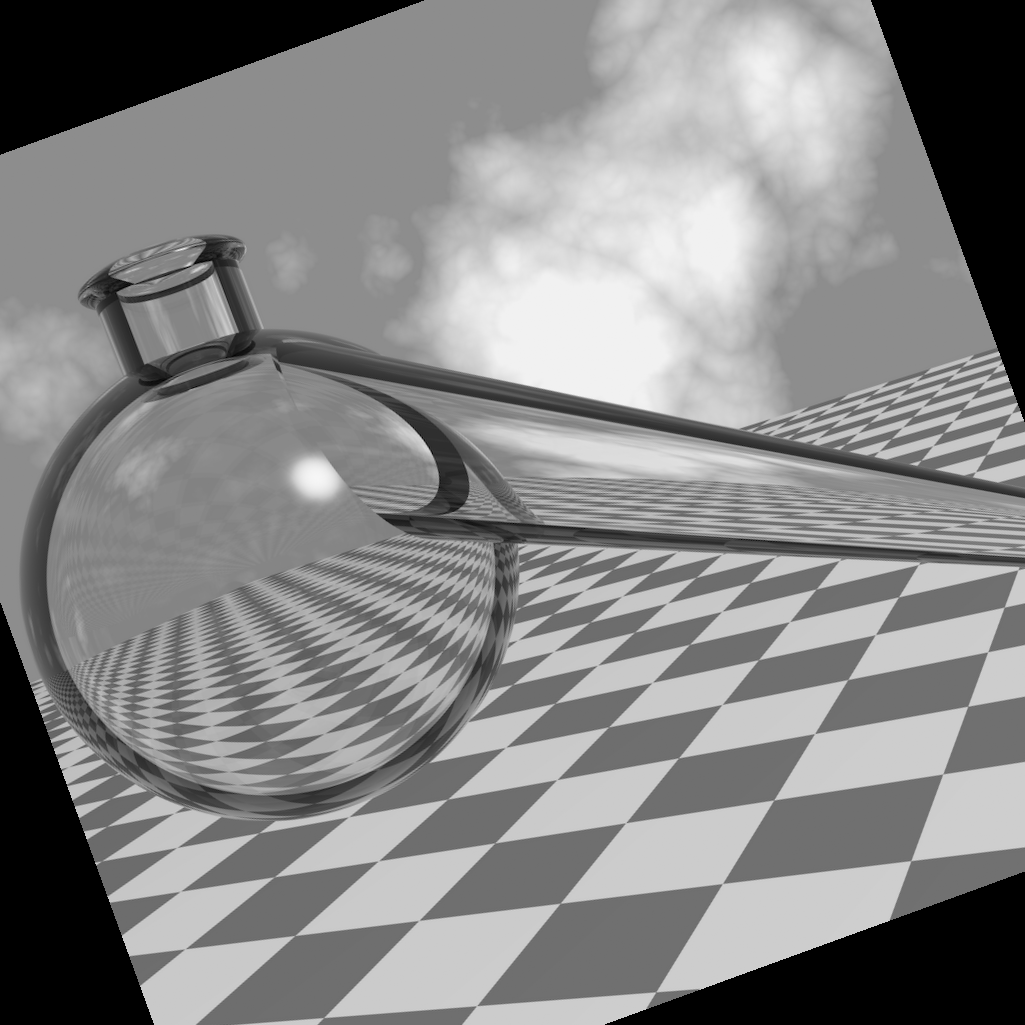
\includegraphics[width=\linewidth]{./images/6/rotate_20_bl.png}}
    \caption{\small{Rotate 20° bilinear}}
    \end{minipage}
\end{figure}

\pagebreak

\begin{figure}[!htb]\centering
    \begin{minipage}{0.6\textwidth}
        \frame{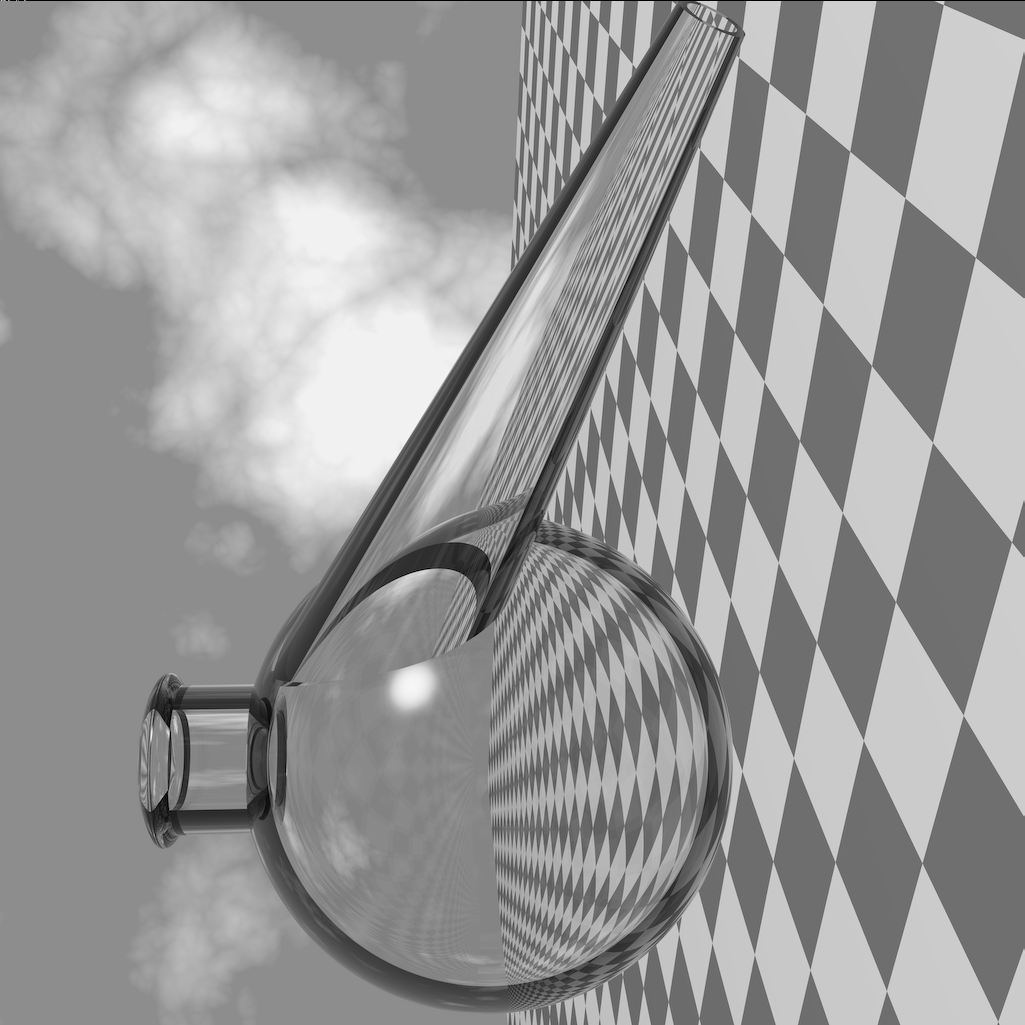
\includegraphics[width=\linewidth]{./images/6/rotate_90_nn.png}}
        \caption{\small{Rotate 90° nearest}}
    \end{minipage}
\end{figure}

\begin{figure}[!htb]\centering
    \begin{minipage}{0.6\textwidth}
    \frame{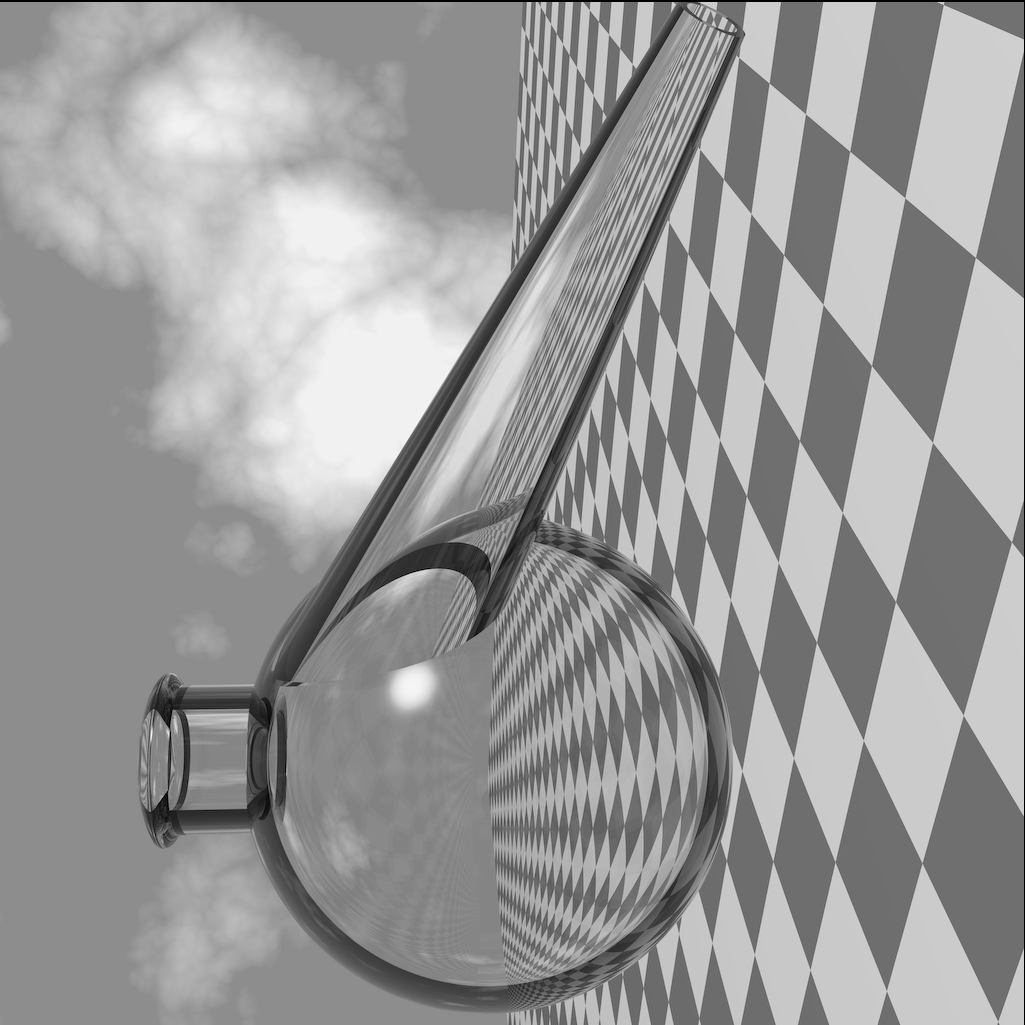
\includegraphics[width=\linewidth]{./images/6/rotate_90_bl.png}}
    \caption{\small{Rotate 90° bilinear}}
    \end{minipage}
\end{figure}


\pagebreak

\begin{figure}[!htb]\centering
    \begin{minipage}{0.6\textwidth}
        \frame{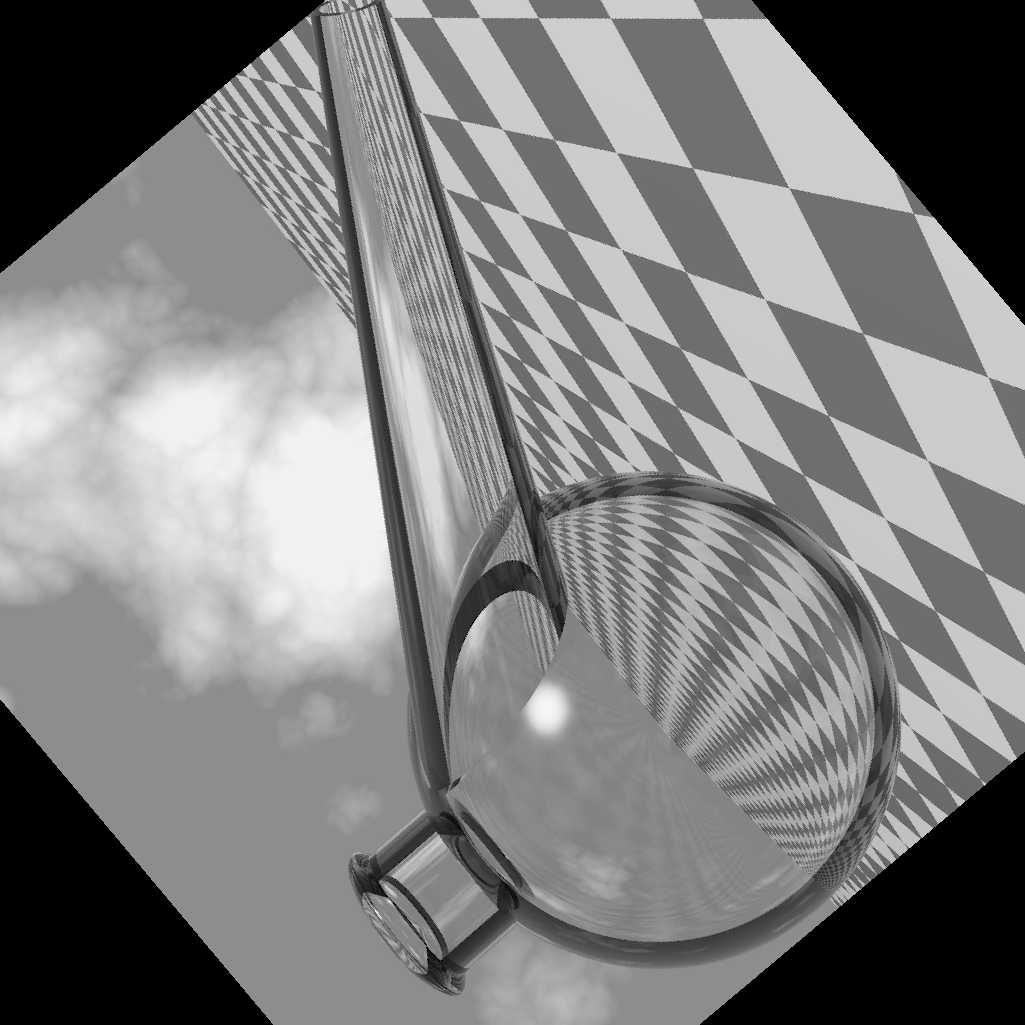
\includegraphics[width=\linewidth]{./images/6/rotate_130_nn.png}}
        \caption{\small{Rotate 130° nearest}}
    \end{minipage}
\end{figure}

\begin{figure}[!htb]\centering
    \begin{minipage}{0.6\textwidth}
    \frame{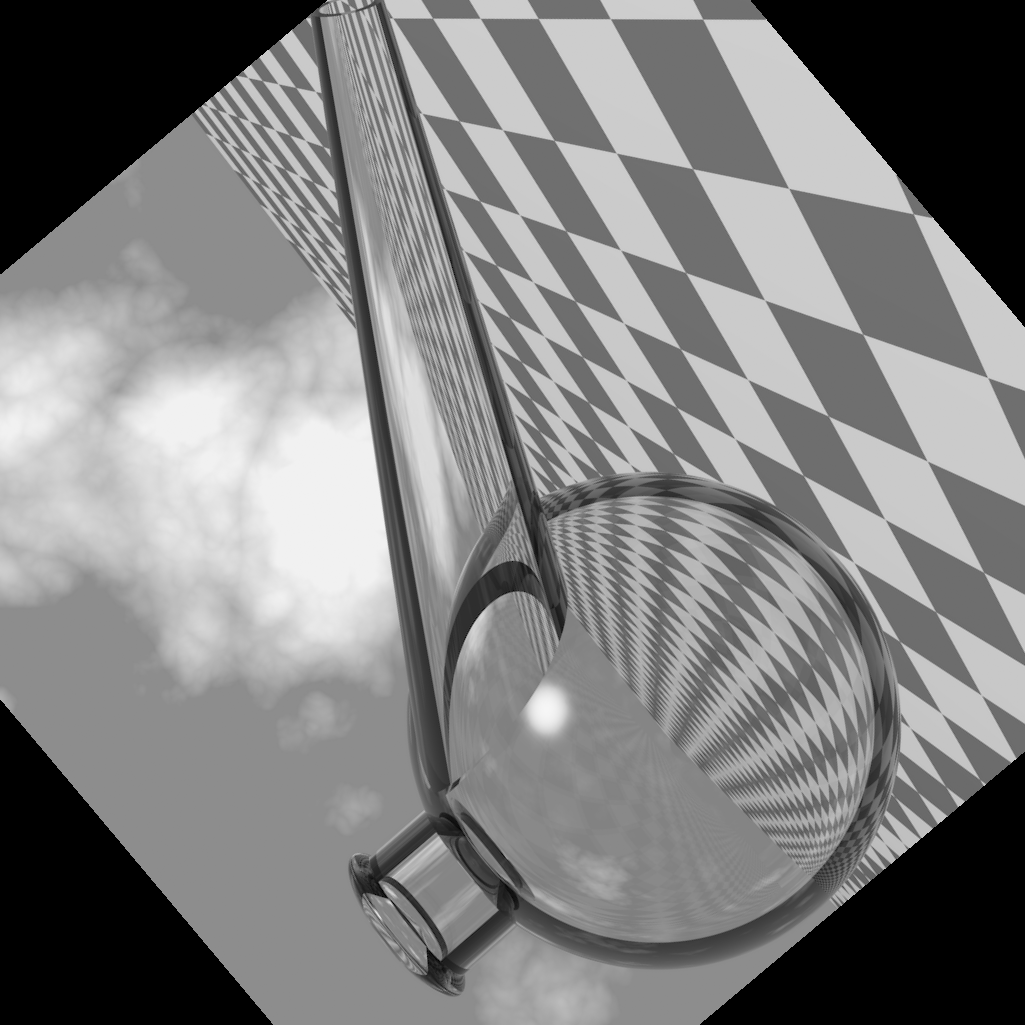
\includegraphics[width=\linewidth]{./images/6/rotate_130_bl.png}}
    \caption{\small{Rotate 130° bilinear}}
    \end{minipage}
\end{figure}

\pagebreak

\section{Scaling}

\begin{figure}[!htb]\centering
    \begin{minipage}{0.6\textwidth}
        \frame{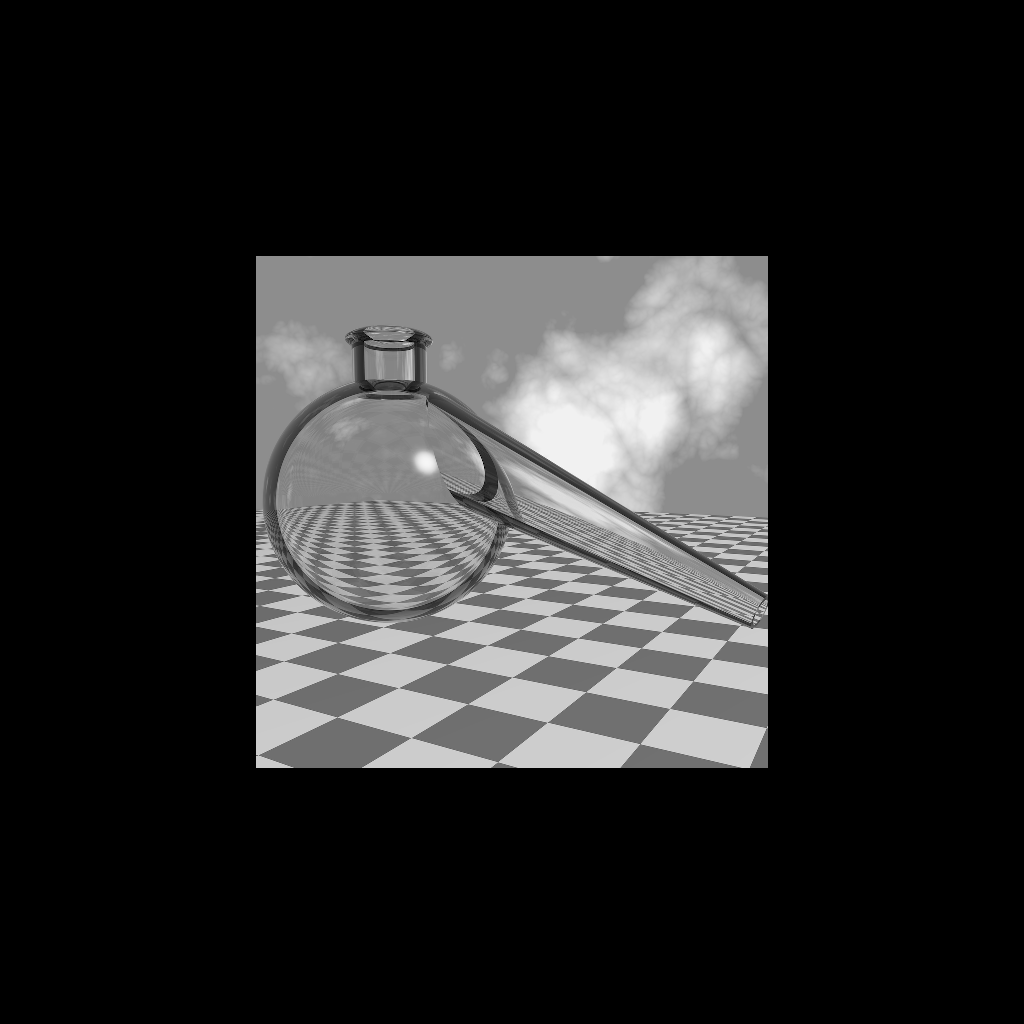
\includegraphics[width=\linewidth]{./images/6/scale_0_5_nn.png}}
        \caption{\small{Scaling 0.5 nearest}}
    \end{minipage}
\end{figure}

\begin{figure}[!htb]\centering
    \begin{minipage}{0.6\textwidth}
    \frame{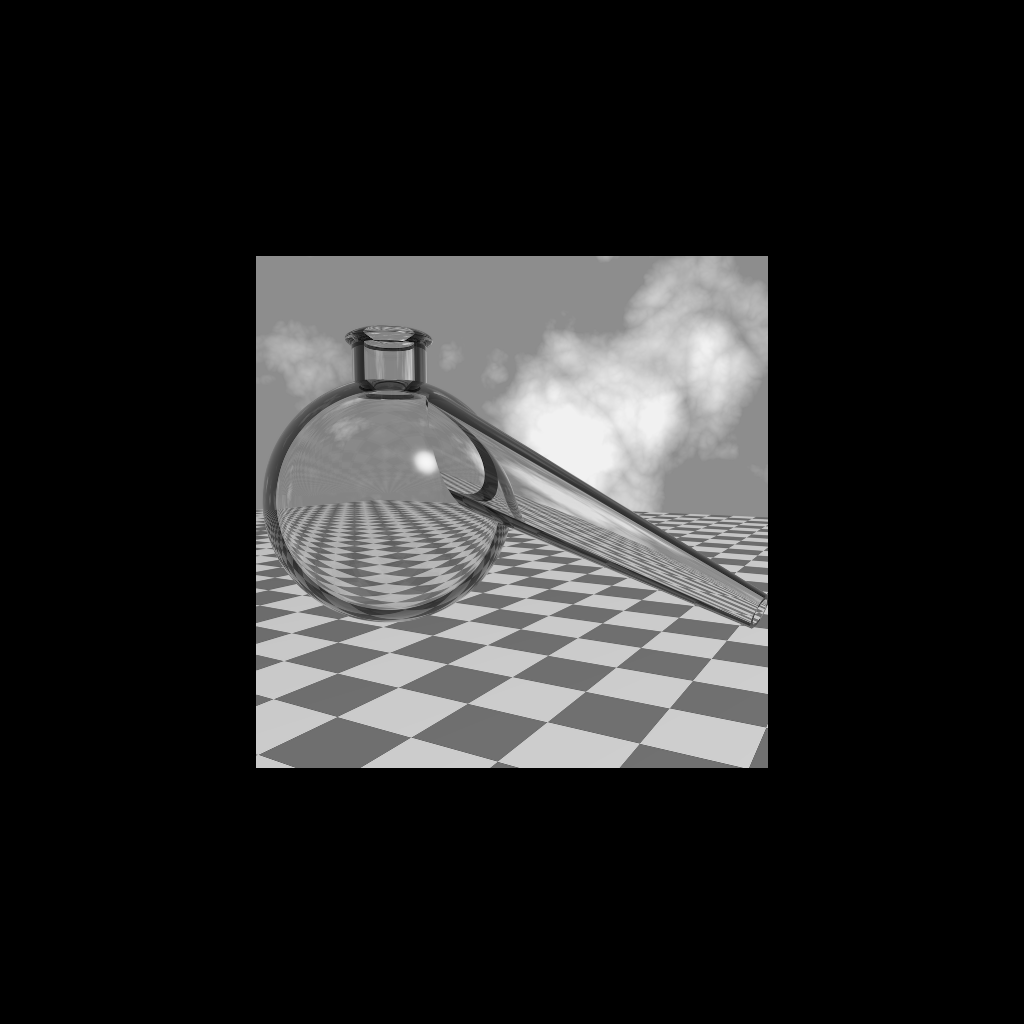
\includegraphics[width=\linewidth]{./images/6/scale_0_5_bl.png}}
    \caption{\small{Scaling 0.5 bilinear}}
    \end{minipage}
\end{figure}

\pagebreak

\begin{figure}[!htb]\centering
    \begin{minipage}{0.6\textwidth}
        \frame{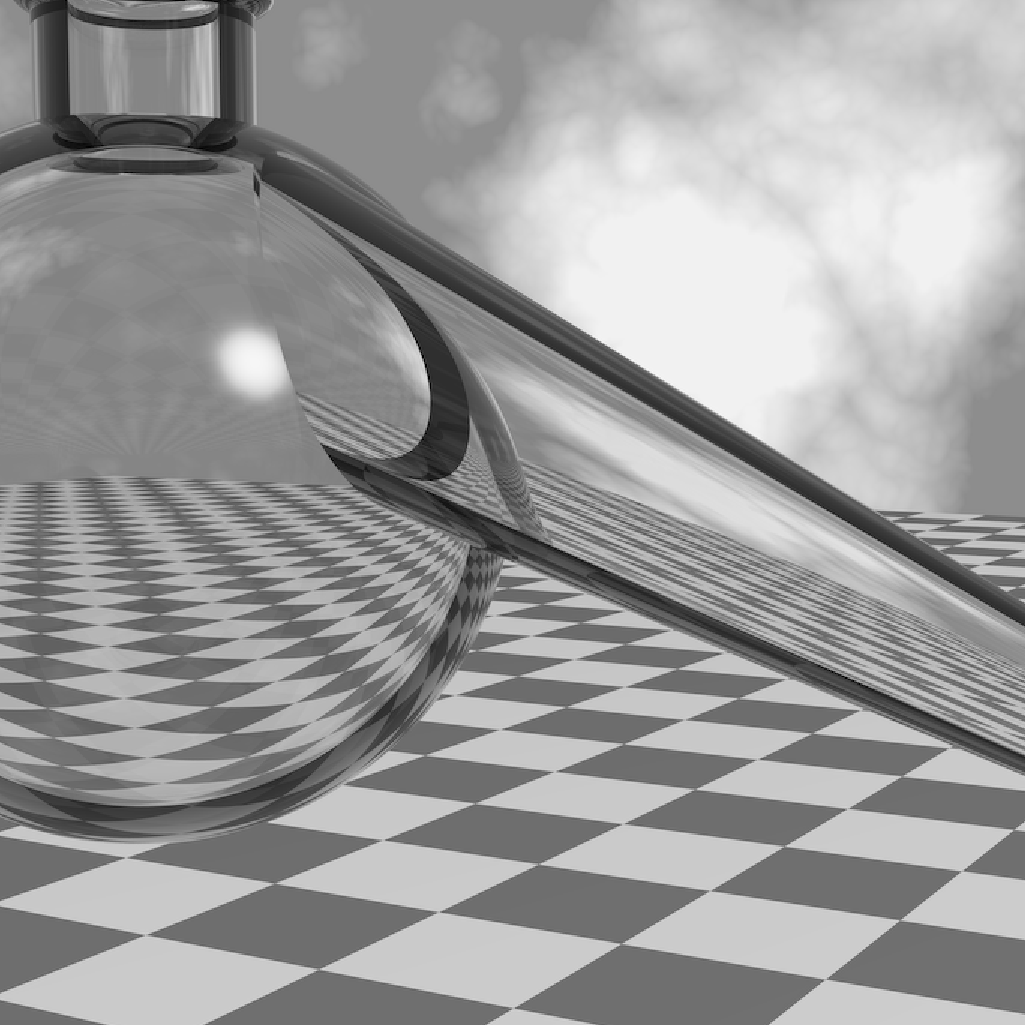
\includegraphics[width=\linewidth]{./images/6/scale_1_5_nn.png}}
        \caption{\small{Scaling 1.5 nearest}}
    \end{minipage}
\end{figure}

\begin{figure}[!htb]\centering
    \begin{minipage}{0.6\textwidth}
    \frame{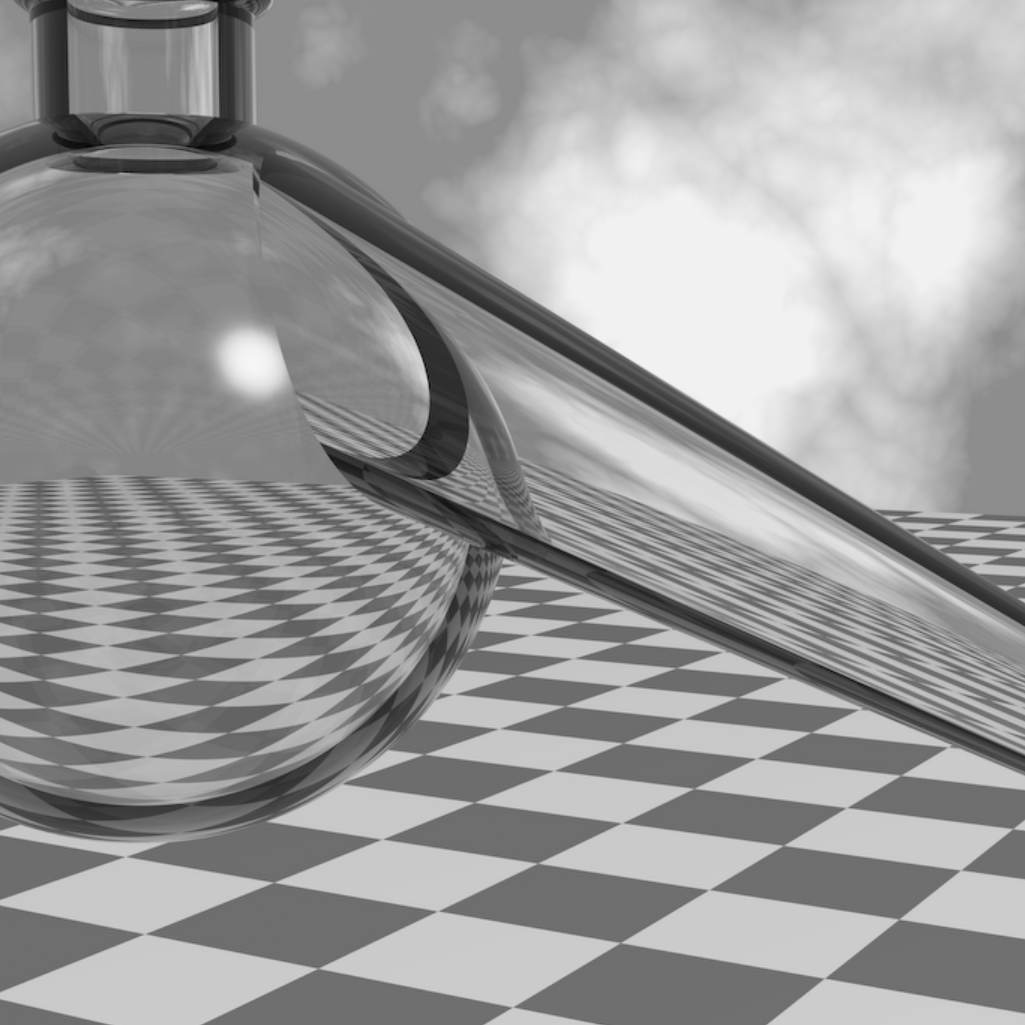
\includegraphics[width=\linewidth]{./images/6/scale_1_5_bl.png}}
    \caption{\small{Scaling 1.5 bilinear}}
    \end{minipage}
\end{figure}

\pagebreak

\begin{figure}[!htb]\centering
    \begin{minipage}{0.6\textwidth}
        \frame{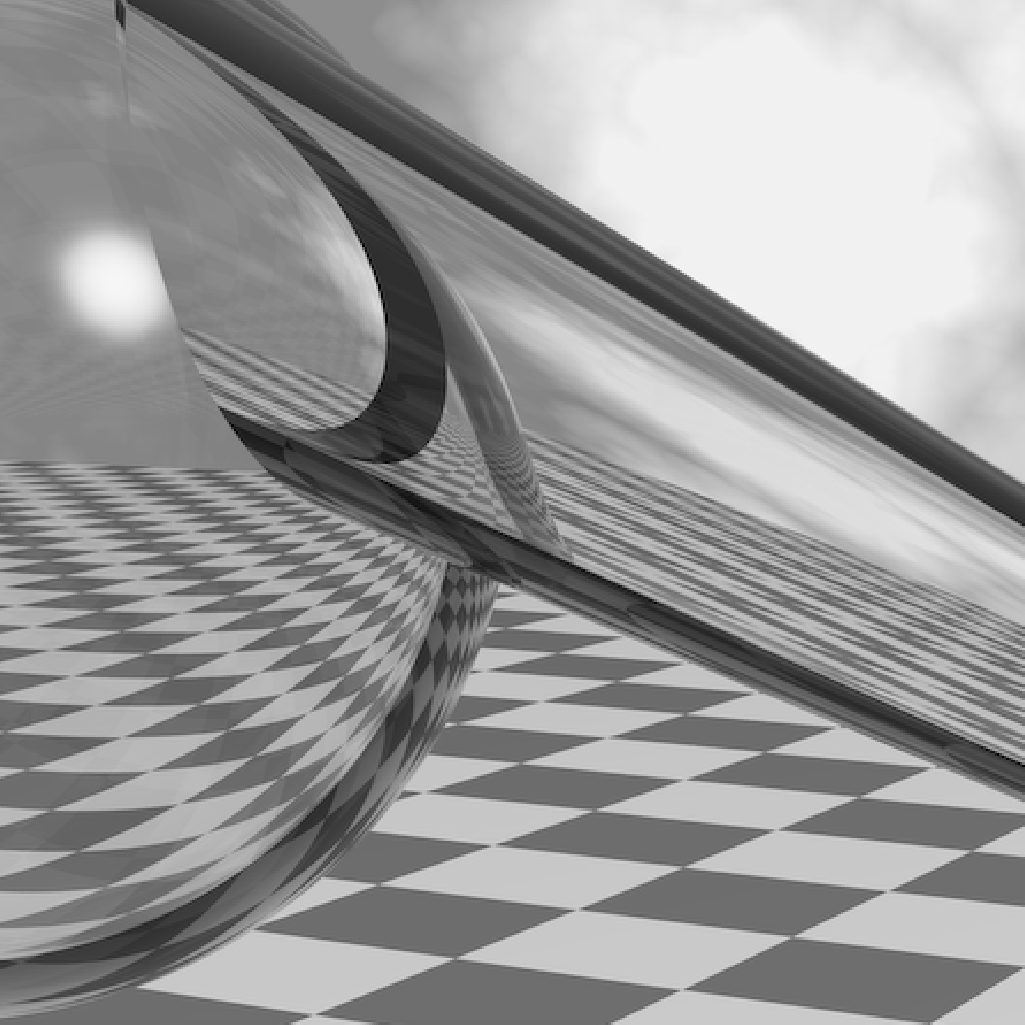
\includegraphics[width=\linewidth]{./images/6/scale_2_3_nn.png}}
        \caption{\small{Scaling 2.3 nearest}}
    \end{minipage}
\end{figure}

\begin{figure}[!htb]\centering
    \begin{minipage}{0.6\textwidth}
    \frame{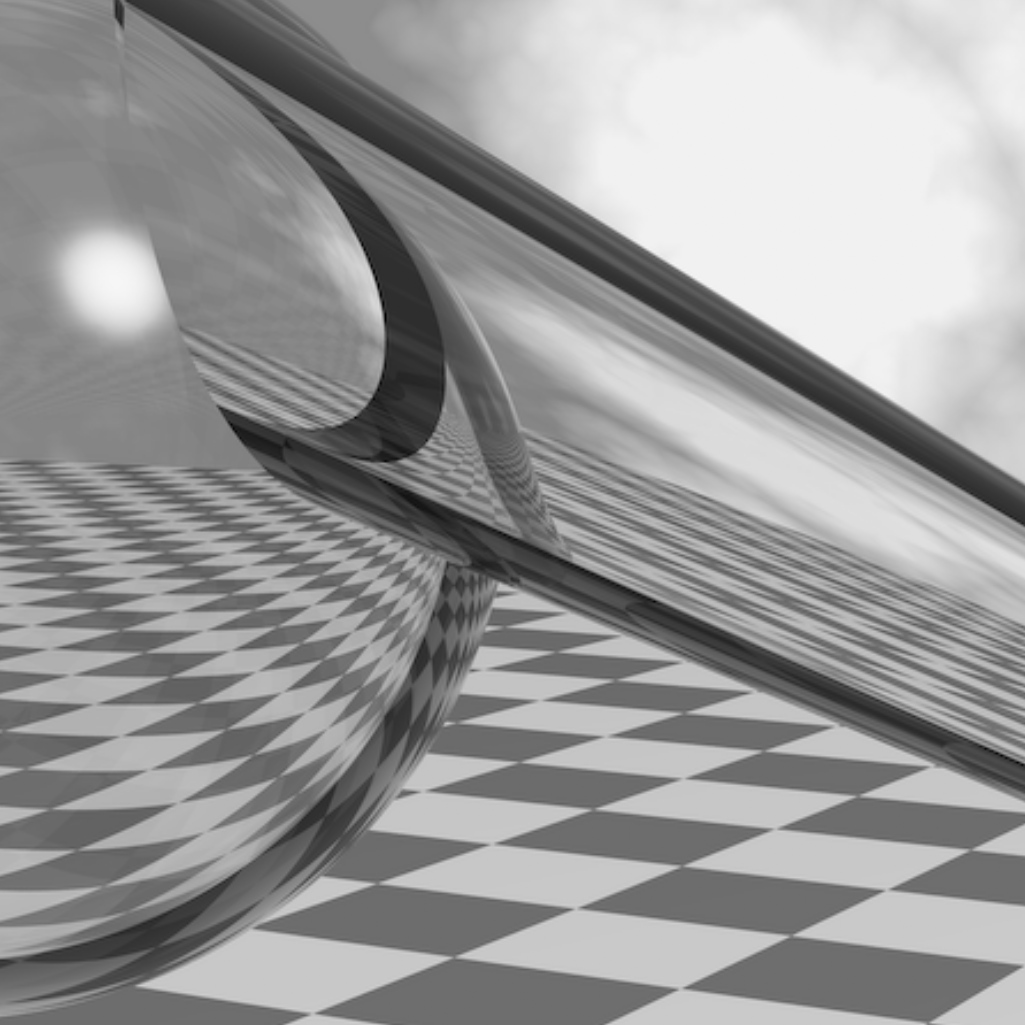
\includegraphics[width=\linewidth]{./images/6/scale_2_3_bl.png}}
    \caption{\small{Scaling 2.3 bilinear}}
    \end{minipage}
\end{figure}
